\section{Akceptowanie i odrzucanie zleceń}

Utworzone przez klienta zlecenie wysyłane jest do wszystkich wykonawców, którzy świadczą żądaną usługę w pobliżu zadanej lokalizacji. Mogą je wówczas zaakceptować lub odrzucić. W tej sekcji zaprezentowane zostaną elementy, które to umożliwiają. Odpowiednie ekrany przedstawiono na rysunku \ref{fig:expert-jobs}.

\begin{figure}[ht]
  \captionsetup[subfigure]{justification=centering}
  \centering
  \begin{subfigure}[t]{0.32\textwidth}
    \centering
    \fbox{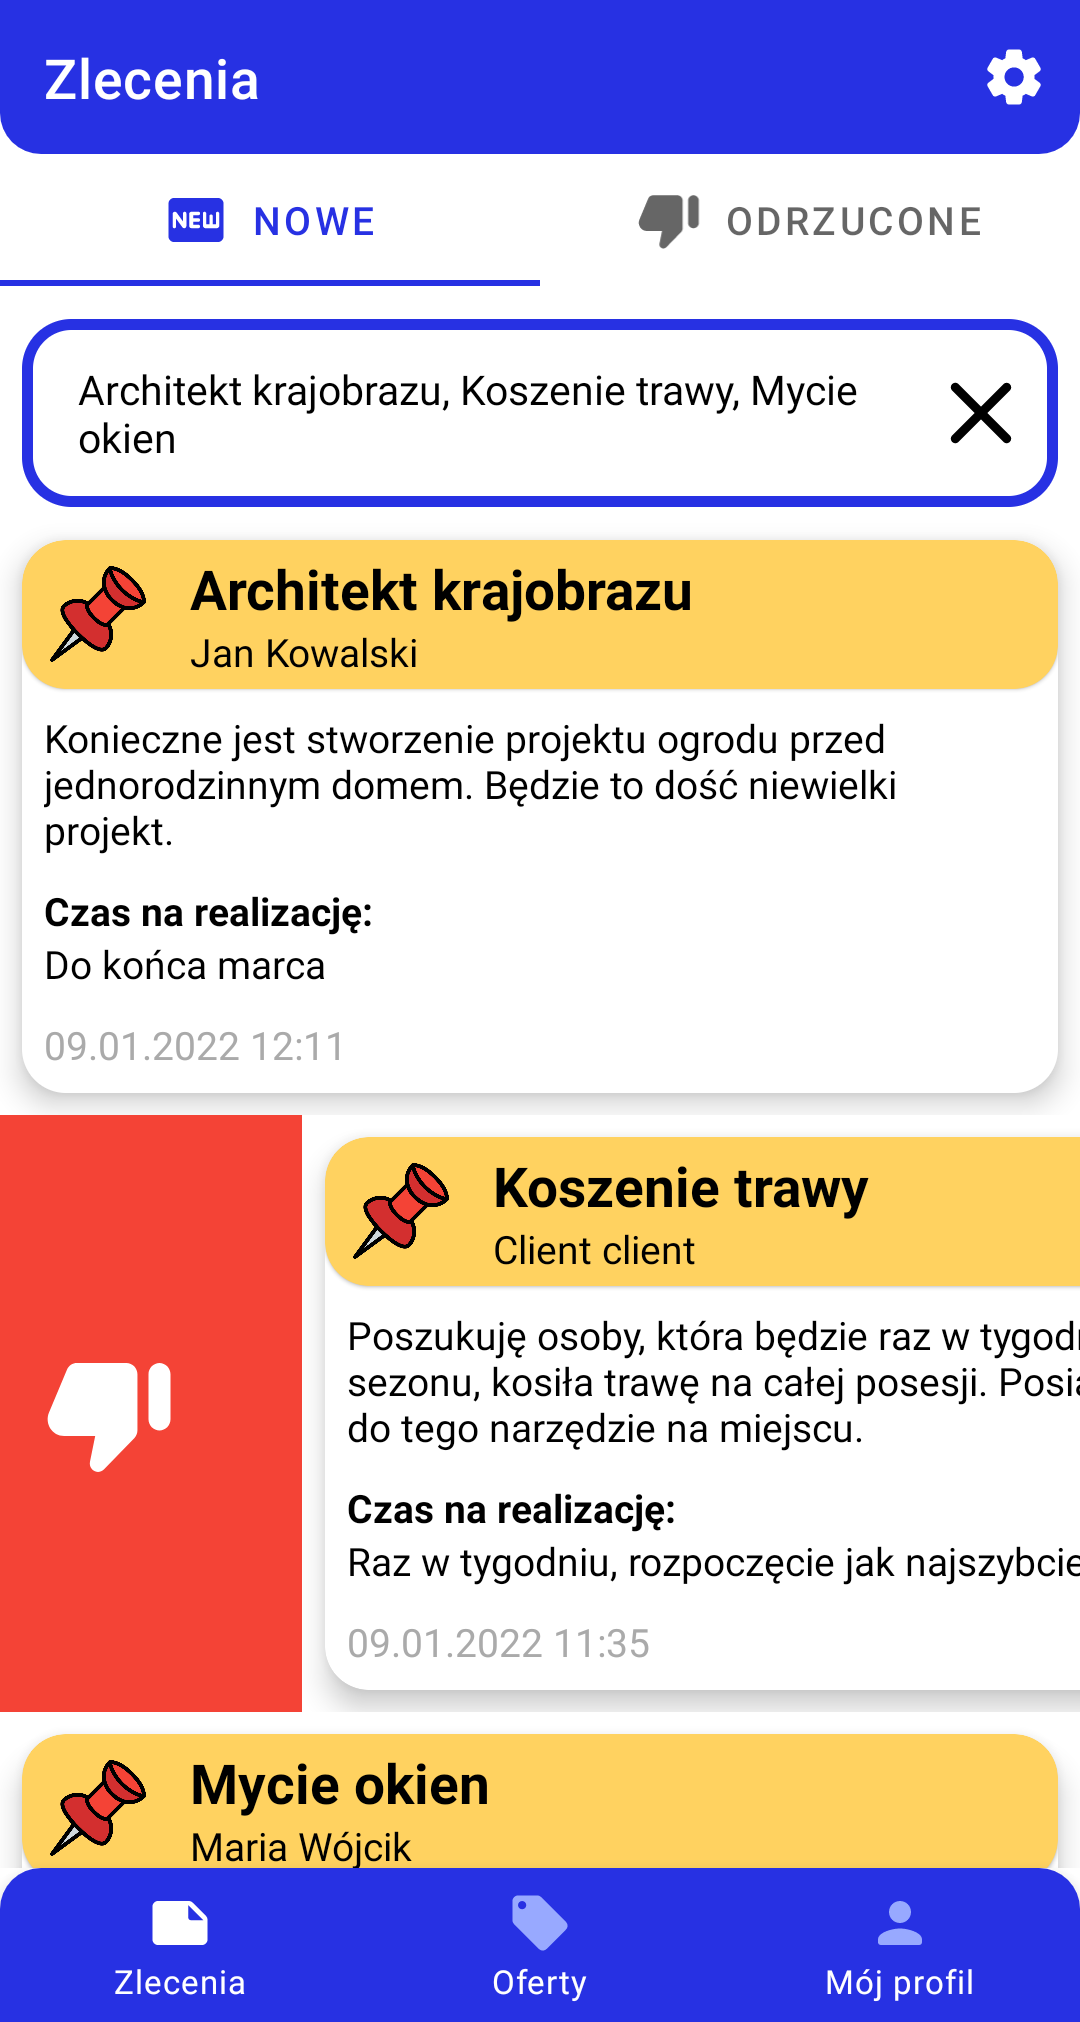
\includegraphics[width=0.97\linewidth]{screens/expert_jobs_swap.png}}
    \caption{Widok dostępnych dla wykonawcy zleceń}
  \end{subfigure}
  \begin{subfigure}[t]{0.32\textwidth}
    \centering
    \fbox{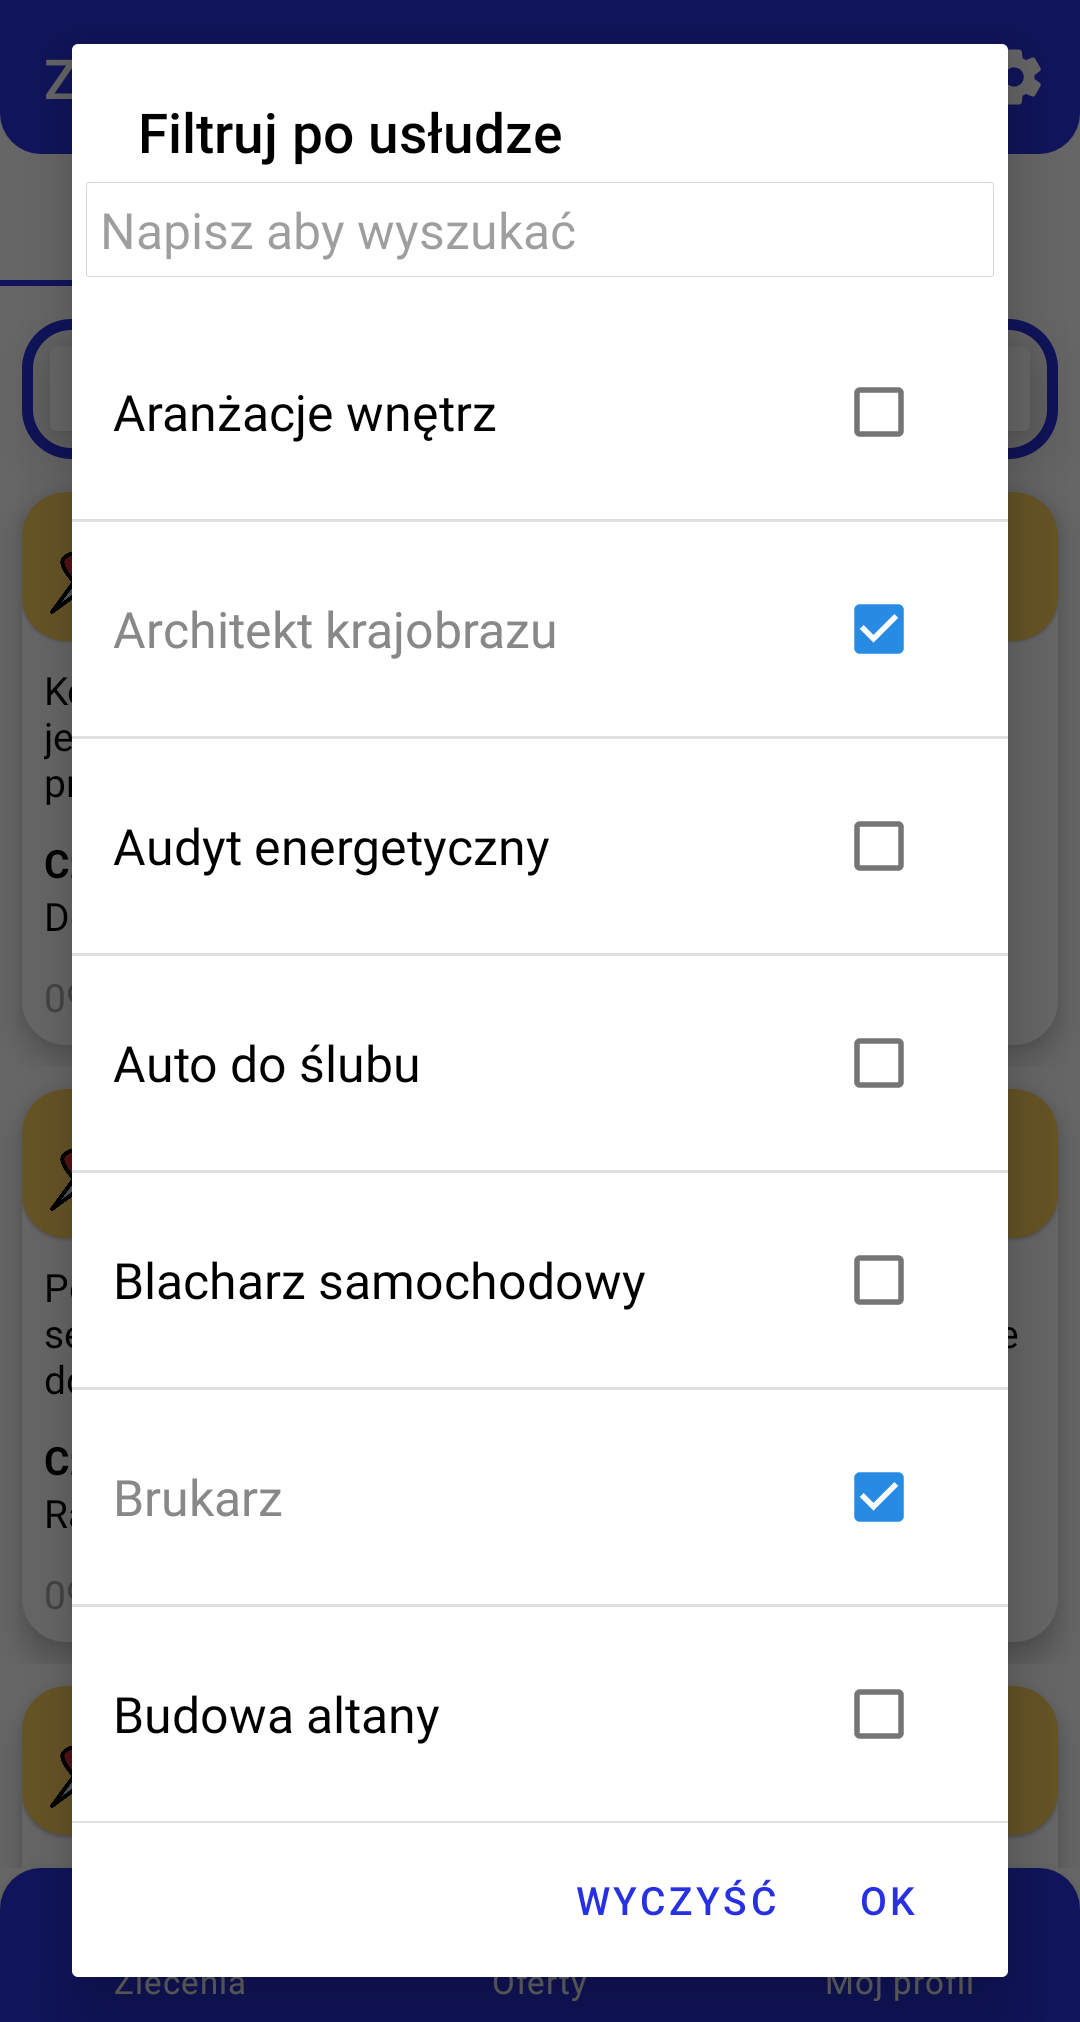
\includegraphics[width=0.97\linewidth]{screens/expert_jobs_filter.png}}
    \caption{Widok okna dialogowego filtrowania}
  \end{subfigure}
  \begin{subfigure}[t]{0.32\textwidth}
    \centering
    \fbox{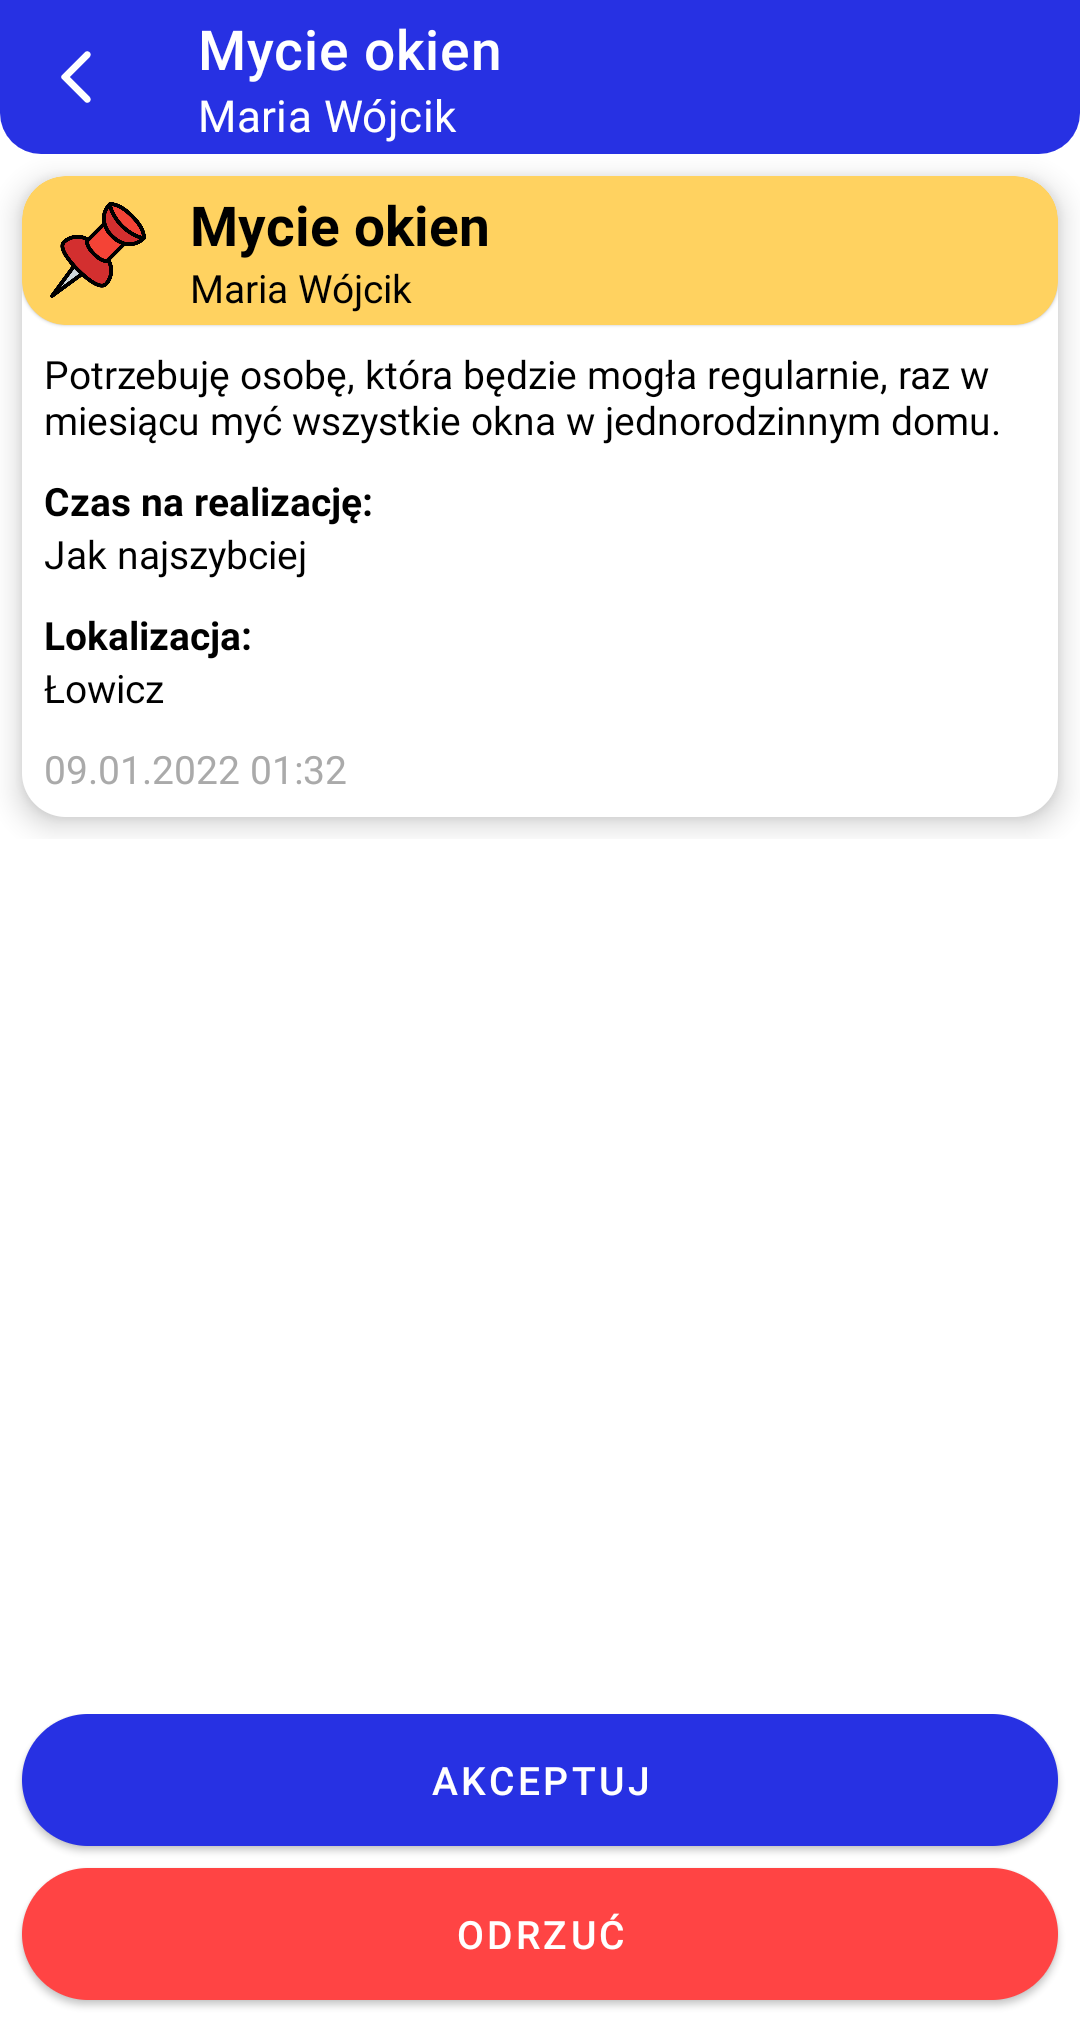
\includegraphics[width=0.97\linewidth]{screens/expert_job.png}}
    \caption{Widok szczegółów zlecenia}
  \end{subfigure}
  \caption{Ekrany umożliwiające akceptowanie i odrzucanie zleceń przez wykonawcę}
  \label{fig:expert-jobs}
\end{figure}

Dostępne dla wykonawcy zlecenia zostały podzielone na dwie kategorie: nowe oraz odrzucone. Można pomiędzy nimi przełączać się z wykorzystaniem zakładek. Dzięki temu, gdy zlecenie zostanie odrzucone, to nie znika bezpowrotnie. Zostaje jedynie przeniesione do kategorii odrzuconych, skąd wykonawca może je przyjąć wtedy, gdy jednak zmieni zdanie. Może się tak zdarzyć na przykład, gdy skończy bieżącą pracę szybciej, niż to przewidywał.

Lista zleceń może być długa, z tego powodu podczas implementacji zastosowano technikę zwaną stronicowaniem. Umożliwia ona pobieranie z bazy danych jedynie tych elementów, które w danej chwili są widoczne na ekranie. Pozwala to zmniejszyć transfer informacji i koszty generowane przez Firebase. 

Aby ułatwić wykonawcom przeszukiwanie zleceń dodano funkcję filtrowania za pomocą nazw usług. Odpowiedzialny za to komponent znajduje się na szczycie listy i jego kliknięcie otwiera okno dialogowe. Są w nim umieszczone wszystkie świadczone usługi i można dokonać ich wielokrotnego wyboru. 

Wybranie konkretnego zlecenia z listy przenosi użytkownika do ekranu szczegółów. Jeżeli jest ono nowe, to ekran zawiera przyciski do akceptacji i odrzucenia. Jeżeli natomiast jest już odrzucone, to widoczny jest jedynie pierwszy przycisk. Kliknięcie go powoduje przyjęcie zlecenia i usunięcie z listy dostępnych. 

Przewidziana została również funkcja szybkiego odrzucenia zlecenia. Polega ona na prostym przeciągnięciu wybranego elementu na liście w prawo. Stwierdzono bowiem, że już widoczne tam informacje mogą skłonić do tego wykonawcę i nie trzeba go zmuszać do otwierania ekranu szczegółów.